\chapter{Grundlagen}

In diesem Kapitel wird das Wissen vermittelt, welches benötigt wird um zu Verstehen, wie \acp{NNUE} im Rahmen von Schachcomputern funktionieren. Zuerst wird die Evaluation, wie sie in herkömmlichen Schachcomputern funktioniert erklärt, auch \ac{HCE} genannt.

\section{Hand-crafted Evaluation}
\label{chap:HCE}

Die Evaluation einer Schachposition ist eine heuristische Methode der Position einen numerischen Wert zuzuordnen. Hätten wir unendliche Ressourcen könnten wir aus jeder Position alle mögliche Zugfolgen sehen und der Positionen einer der drei Werte: -1 (Verlust), 0 (remis), 1 (Gewinn) geben. In der Realität ist es nicht möglich den exakten Wert der Stellung zu kennen, deshalb wird in der \ac{HCE} versucht anhand von Menschen festgelegten Kriterien einen Wert der Position zuzuordnen. 
Vor der Verbreitung von \acp{NN}, war \ac{HCE} die einzige Form der Positions-Evaluation. 

\section{Neuronale Netze}

\tikzset{
  every neuron/.style={
    circle,
    draw,
    minimum size=1cm
  },
  neuron missing/.style={
    draw=none, 
    scale=4,
    text height=0.333cm,
    execute at begin node=\color{black}$\vdots$
  },
}

\begin{figure}
  \centering
  % taken from: https://tex.stackexchange.com/questions/153957/drawing-neural-network-with-tikz
  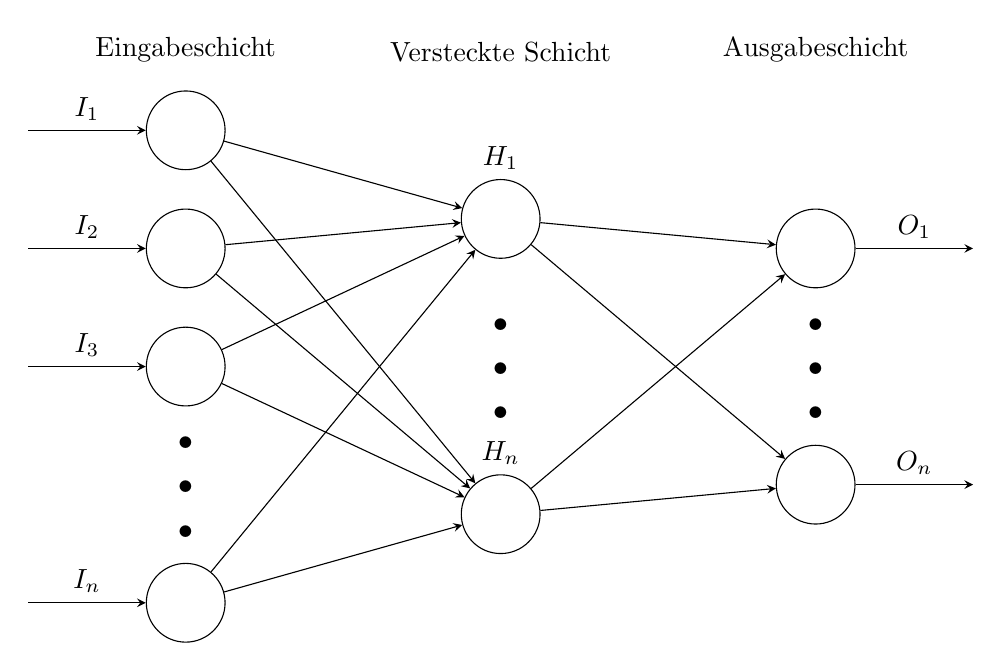
\begin{tikzpicture}[x=2cm, y=1.5cm, >=stealth]
  
  \foreach \m/\l [count=\y] in {1,2,3,missing,4}
    \node [every neuron/.try, neuron \m/.try] (input-\m) at (0,2.5-\y) {};
  
  \foreach \m [count=\y] in {1,missing,2}
    \node [every neuron/.try, neuron \m/.try ] (hidden-\m) at (2,2-\y*1.25) {};
  
  \foreach \m [count=\y] in {1,missing,2}
    \node [every neuron/.try, neuron \m/.try ] (output-\m) at (4,1.5-\y) {};
  
  \foreach \l [count=\i] in {1,2,3,n}
    \draw [<-] (input-\i) -- ++(-1,0)
      node [above, midway] {$I_\l$};
  
  \foreach \l [count=\i] in {1,n}
    \node [above] at (hidden-\i.north) {$H_\l$};
  
  \foreach \l [count=\i] in {1,n}
    \draw [->] (output-\i) -- ++(1,0)
      node [above, midway] {$O_\l$};
  
  \foreach \i in {1,...,4}
    \foreach \j in {1,...,2}
      \draw [->] (input-\i) -- (hidden-\j);
  
  \foreach \i in {1,...,2}
    \foreach \j in {1,...,2}
      \draw [->] (hidden-\i) -- (output-\j);
  
  \foreach \l [count=\x from 0] in {Eingabeschicht, Versteckte Schicht, Ausgabeschicht}
    \node [align=center, above] at (\x*2,2) {\l};
  
  \end{tikzpicture}
  \caption{Ein exemplarisches \acl{NN} mit }
  \label{grundlagen:beispiel-nn}
\end{figure}

\Acp{KNN} oder einfach \acp{NN} genannt, sind Computer Systeme, die dem biologischen Vorbild des Gehirns nachempfunden sind. In Abbildung \autoref{grundlagen:beispiel-nn} ist ein einfaches \acl{NN} zu sehen. Es besteht aus 

\ac{NN} bestehen aus

\subsection{Das Neuron}

% neuronen wie sie im nerfen systems eines menschen vorhanden sind
Das Neuron ist der elementare Bestandteil eines \acp{NN}.
Um Neuronen eines \acp{NN} zu verstehen, schauen wi

\subsection{Backpropagation}
% viel muss man davon nicht kennen, da pytorch das übernimmt (automatic through automatic differentiation)
Als Backpropagation wird das Verfahren der Fehlerrückführung beschrieben. Es gehört zu der Familie der überwachten Lernverfahren

% the forward pass gives you the error and the backpropagation computes the gradiants and based on the gradiants the optimization algorithm ajusts the weights, the learing rate is the speed at witch changes occure

\subsection{Convolutional Neural Networks}
% kann vl entfernt werden (schau am ende ob man es noch braucht (seiten))
% nur ein kurzer exkurs da es in andern neuronalen netzen für schach computer verwendet wird


\subsection{Loss funcntions}


\subsection{Quantisierung}

Quantisierung ist ein Signalverarbeitungsverfahren, bei welchem Eingabewerte auf eine vorher festgelegte kleinere Menge von Ausgabewerten abgebildet wird. Ein simples Beispiel für Quantisierung ist das Abbilden von rationalen Zahlen auf ganze Zahlen, hierfür müssen die rationalen Zahlen zu der nächsten ganzen Zahl gerundet werden. Im Bereich der Informatik werden für Gleitkomma Eingabewerte oft Festkommazahlen oder Ganzzahlen als Ausgabewerte gewählt \cite{Gysel2016}. Egal wie und welche die Quantisierung stattfindet, das Ziel ist es weniger Speicherkapazität und weniger Berechnungszeit zu benötigen mit minimalen Präzisionsverlust.

% was für für quantisierungs schemen gibt es?

Dieses Verfahren eignet sich gut für Anwendungsgebiete mit wenig Speicher- und Rechenkapazität, wie beispielsweise der Einsatz von \acp{NN} bei Mobilgeräten \cite{MaQuantization2019, Gysel2016}. Der Grund dafür ist zweierlei. Erstens sorgt Quantisierung dafür, dass weniger Platz im cache der CPU gebraucht wird, wodurch weniger Schreib- und Lesezugriffe ausgeführt werden und somit die Berechnung schneller ist. Zweitens ermöglicht die Abbildung auf ganzzahlige Typen einen Performance-Gewinn, durch die Verwendung von Prozessor internen Recheneinheiten die beispielsweise \ac{SIMD} unterstützen.

Das Problem der Quantisierung ist das Einbauen von \enquote{Fehlern}. Bei \acp{NN} wird oft von Fehler-Kumulierung gesprochen, da bei der Aktivierung eines \acp{NN} in jedem Quantisierten Neuron der Fehler wächst \cite{Park2018}.
% es muss immer für jeden einzelnen anwendungs fall überlegt werden ob es sich lohnt, für nnue 

\section{SIMD}

\ac{SIMD}

% chosing what SIMD instruction set to use:
% depends on the hardware ur using, some SIMD is only present in server grade cpus
% vl arbeit raussuchen die einen vergleich zwischen den SIMD instruction sets macht und zitieren

\subsection{Memory Alignment}

